%----------Kimberli's LaTeX template----------

%--- Preamble ---

\documentclass{article}

\usepackage{amsmath}
\usepackage{mathtools}
\usepackage{amssymb}
\usepackage{fancyhdr} 
\usepackage{fullpage}
\usepackage{graphicx}
\usepackage{pgfplots}
\usepackage{hyperref} 
\usepackage{parskip}
\usepackage{titlesec}
\usepackage{adjustbox}
\usepackage{multirow}
\pgfplotsset{compat=1.10}

\rhead{\authors}
\lhead{Fall 2015}
\cfoot{\thepage}
\addtolength{\headsep}{15pt}
\pagestyle{fancy}
\setlength{\headheight}{12pt}
\titleformat{\subsubsection}[runin]{}{}{}{}[]
\renewcommand{\arraystretch}{1.5}
%--- The Document & Definitions---

\begin{document}
\newcommand{\class}{Notably Design Document}
\newcommand{\duedate}{November 13, 2015}
\newcommand{\classsection}{6.170 Fall 2015}
\newcommand{\authors}{Vahid Fazel-Rezai, Alex Luh, Akshay Ravikumar, Kimberli Zhong}

%--- Title ---

\begin{center}
~\\[1cm] 
{\huge \class} \\[0.4cm] 
{\large \authors} \\[0.2cm]
{\large \duedate} \\[0.2cm]
{\large \classsection}
\end{center}

\section*{Overview}
\subsection*{Motivation}
Writing notes during class can be a struggle; it can be hard to write detailed notes and follow the lecture at the same time. This leads to both low-quality notes and an incomplete understanding of the material.

For our final project, we are creating Notably, an application for collaboratively creating and curating notes. MIT students will be able to log into the system and join a lecture feed for a particular class; then, they can contribute notes, flag inappropriate posts, and save useful notes to their personal stash. 

Notably aims to achieve the following:

\begin{itemize}
\item  \textbf{To encourage collaboration within an entire class.} 

While there already exist note-taking tools, many of these aren't collaborative. Those that support collaboration (Google Docs, Evernote, etc.), however, are not readily accessible to the entire class; friends have to send each other a link to access the document. With Notably, all the students in a class can easily access its feed, making classwide collaboration effortless.

\item \textbf{To let students absorb more information from a lecture.}

By streamlining the notetaking process with features like keyboard shortcuts and rich Markdown support, students can easily contribute notes without missing too much important information from the lecture. In addition, by working together to add information, students can better absorb the content without meticulously documenting everything.

\item \textbf{To let students efficiently curate their own notes.}

Notably lets students add their own notes, and those of their peers, to a personal stash. This lets students store important information they wish to access in the future, and we hope that the user experience will be rich enough for MIT students to use Notably for all their notetaking needs.

\end{itemize}

We hope that with Notably, MIT students can communicate and learn from each other, fostering the archetypal MIT collaborative spirit while increasing understanding of the course material.

\newpage

\section*{Design Essence}
\subsection*{Concepts}
Snippet
\begin{itemize}
\item Purpose: To allow a user to create a note for a certain topic in a class session (lecture, recitation, etc.)
\item Operational Principle: If a user wants to write down the different ways to structure data in mongo, he or she can create a new snippet containing a table of the pros and cons of the embedded versus relational structures.
\end{itemize}

Stash
\begin{itemize}
\item Purpose: To allow a user to create an organized list of all notes he or she took for a class session
\item Operational Principle: If a user wants to review his or her personal notes for a lecture before an exam, he or she can look at his or her own stash for that lecture.
\end{itemize}

Feed
\begin{itemize}
\item Purpose: To allow a user to see a consolidated list of all notes taken by students in a class session
\item Operational Principle: If a user feels confused about a particular topic during a lecture, he or she can look at the class feed to see if some other student has written a clear and helpful note about that topic.
\end{itemize}

Save
\begin{itemize}
\item Purpose: To allow a user to add a particularly insightful note written by another user to their own lecture notes
\item Operational Principle: If a user sees a really good note for a certain topic in the class feed, he or she can add it to his or her stash for the lecture. Saves also serve as a rating system, since a snippet with many saves is likely to be better quality than a snippet with zero saves.
\end{itemize}

Flag
\begin{itemize}
\item Purpose: To allow a user to mark a note as incorrect or low quality; prevents trolls and spam
\item Operational Principle: If a user sees a snippet in the class feed that is incorrect about some topic or obviously spam, he or she can flag that snippet. If a user has too many flagged snippets, he or she will temporarily lose access to the class feed.
\end{itemize}

Unlocking
\begin{itemize}
\item Purpose: To encourage students to be engaged in class
\item Operational Principle: Upon logging into Notably, a user can only see the top ten snippets in the class feed. If the user wishes to see more of the snippets in the class feed, he or she must contribute three good snippets to unlock access to the entire class feed.
\item Potential Misfit: The concept of unlocking alone doesn't necessarily incentivize students to attend class.
\end{itemize}

\subsection*{Data model}
\begin{center}

\includegraphics[width=6in]{DataModel.png}
\end{center}

Definitions:
\begin{itemize}
\item subscribed\_to indicates that a user is subscribed to feeds in a class
\item has\_sessions denotes which sessions belong to a given class (lectures, recitations, study sessions, etc.)
\item saved\_snippets marks which snippets a user has saved to his/her stash
\item flagged\_by indicates which users have flagged a given snippet as incorrect or spammy
\end{itemize}

Textual constraints:
\begin{itemize}
\item A stash for a given session cannot contain snippets not in that session's feed
\end{itemize}

Insights:
\begin{itemize}
\item The feed is consolidated globally so that every user subscribed to its class can see it, given that they've unlocked the view. 
\item We use a session model to represent each class session. For each session, users can then add notes (snippets) to that session's feed. 
\end{itemize}

\subsection*{Security concerns}

We want notes to be as open as possible within classes, but to make participants comfortable with that we would like to limit access to the notes to MIT students. This also prevents spam from outside users. To do so, we will use a simple MIT certificate authorization system. That is, accessing any page of the system requires an MIT certificate. This also allows us to identify users by Kerberos ID.

We will prevent standard web attacks (XSS, CSRF, etc.) using standard techniques presented in lecture such as input sanitization (e.g. for snippets) and using authorization tokens. We will manage who has access to resources (such as feeds that aren't unlocked) on the server-side to prevent users from being able to access restricted content through HTML sources.

We are assuming attackers are anyone on the Internet (not just MIT students) who do not have access to the server directly but can send any request to any endpoint. We assume only MIT students have MIT certificates.


\subsection*{User interface}

\begin{figure}[h!]
  \caption{Splash page}
  \centering
    
\includegraphics[width=6in]{UI4.png}
\end{figure}

\begin{figure}[h!]
  \caption{Home view}
  \centering
    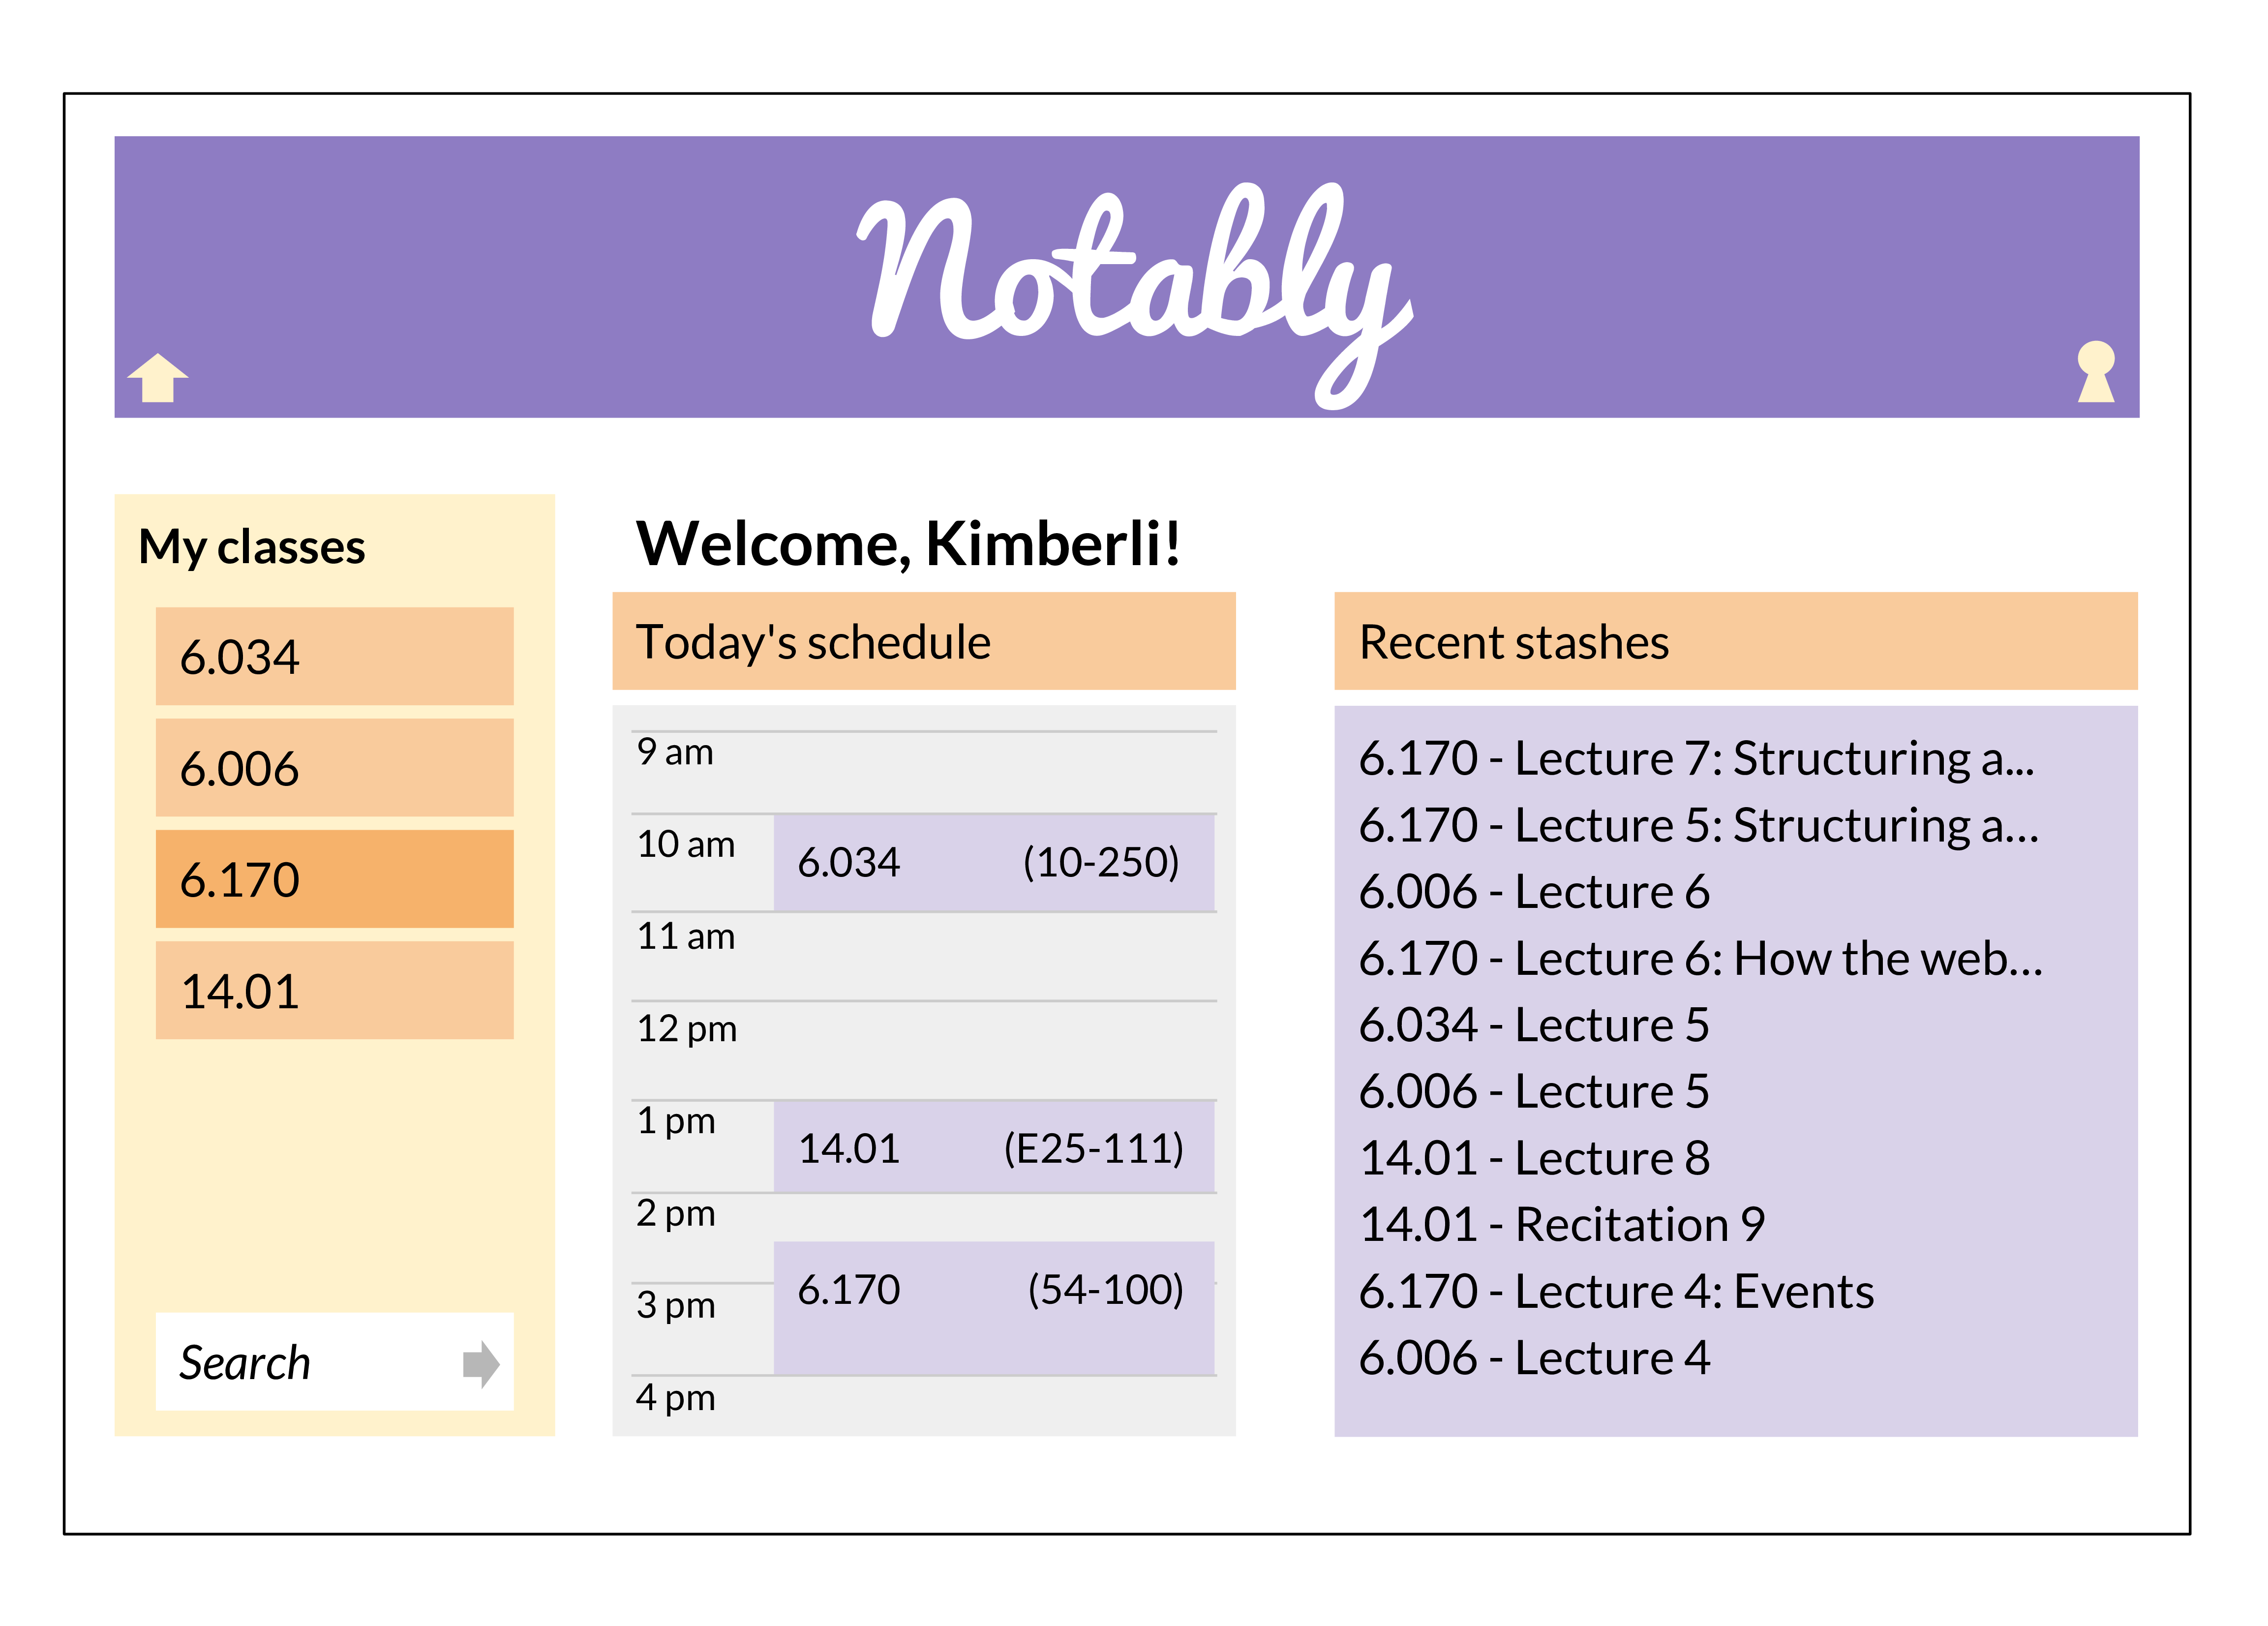
\includegraphics[width=6in]{UI3.png}
\end{figure}

\begin{figure}[h!]
  \caption{Class view}
  \centering
    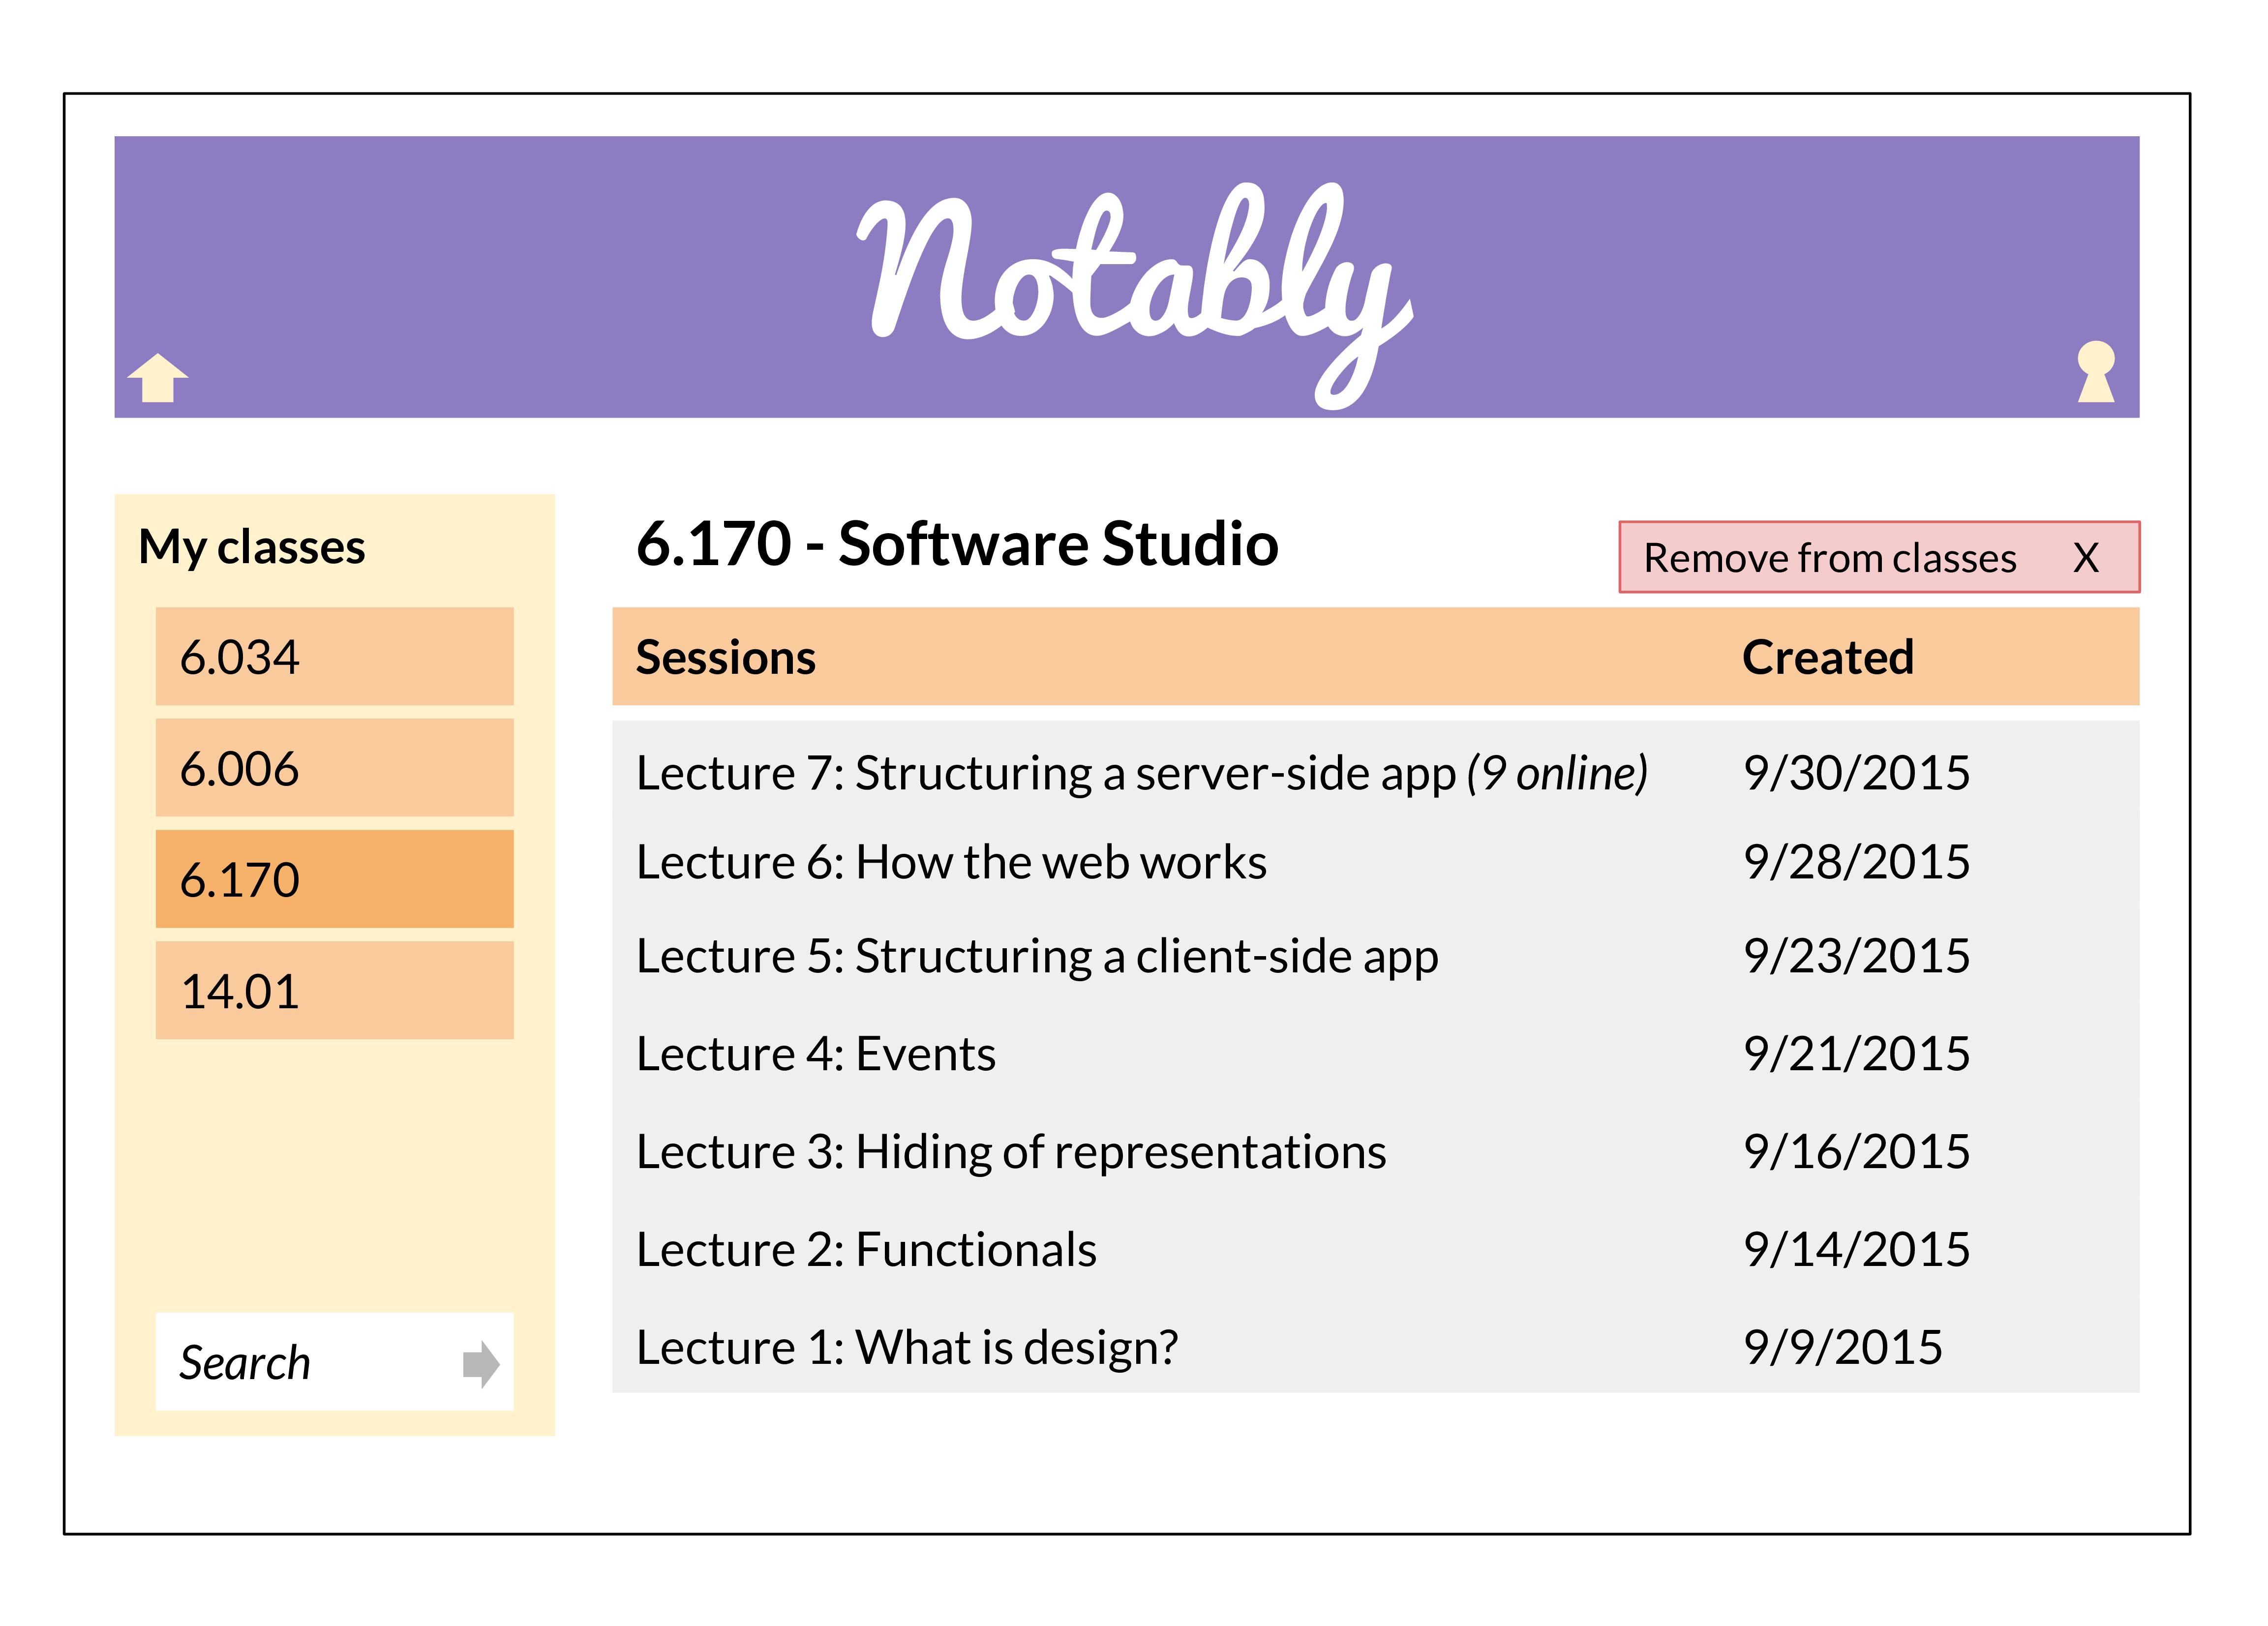
\includegraphics[width=6in]{UI2.png}
\end{figure}

\begin{figure}[h!]
  \caption{Session \& stash view}
  \centering
    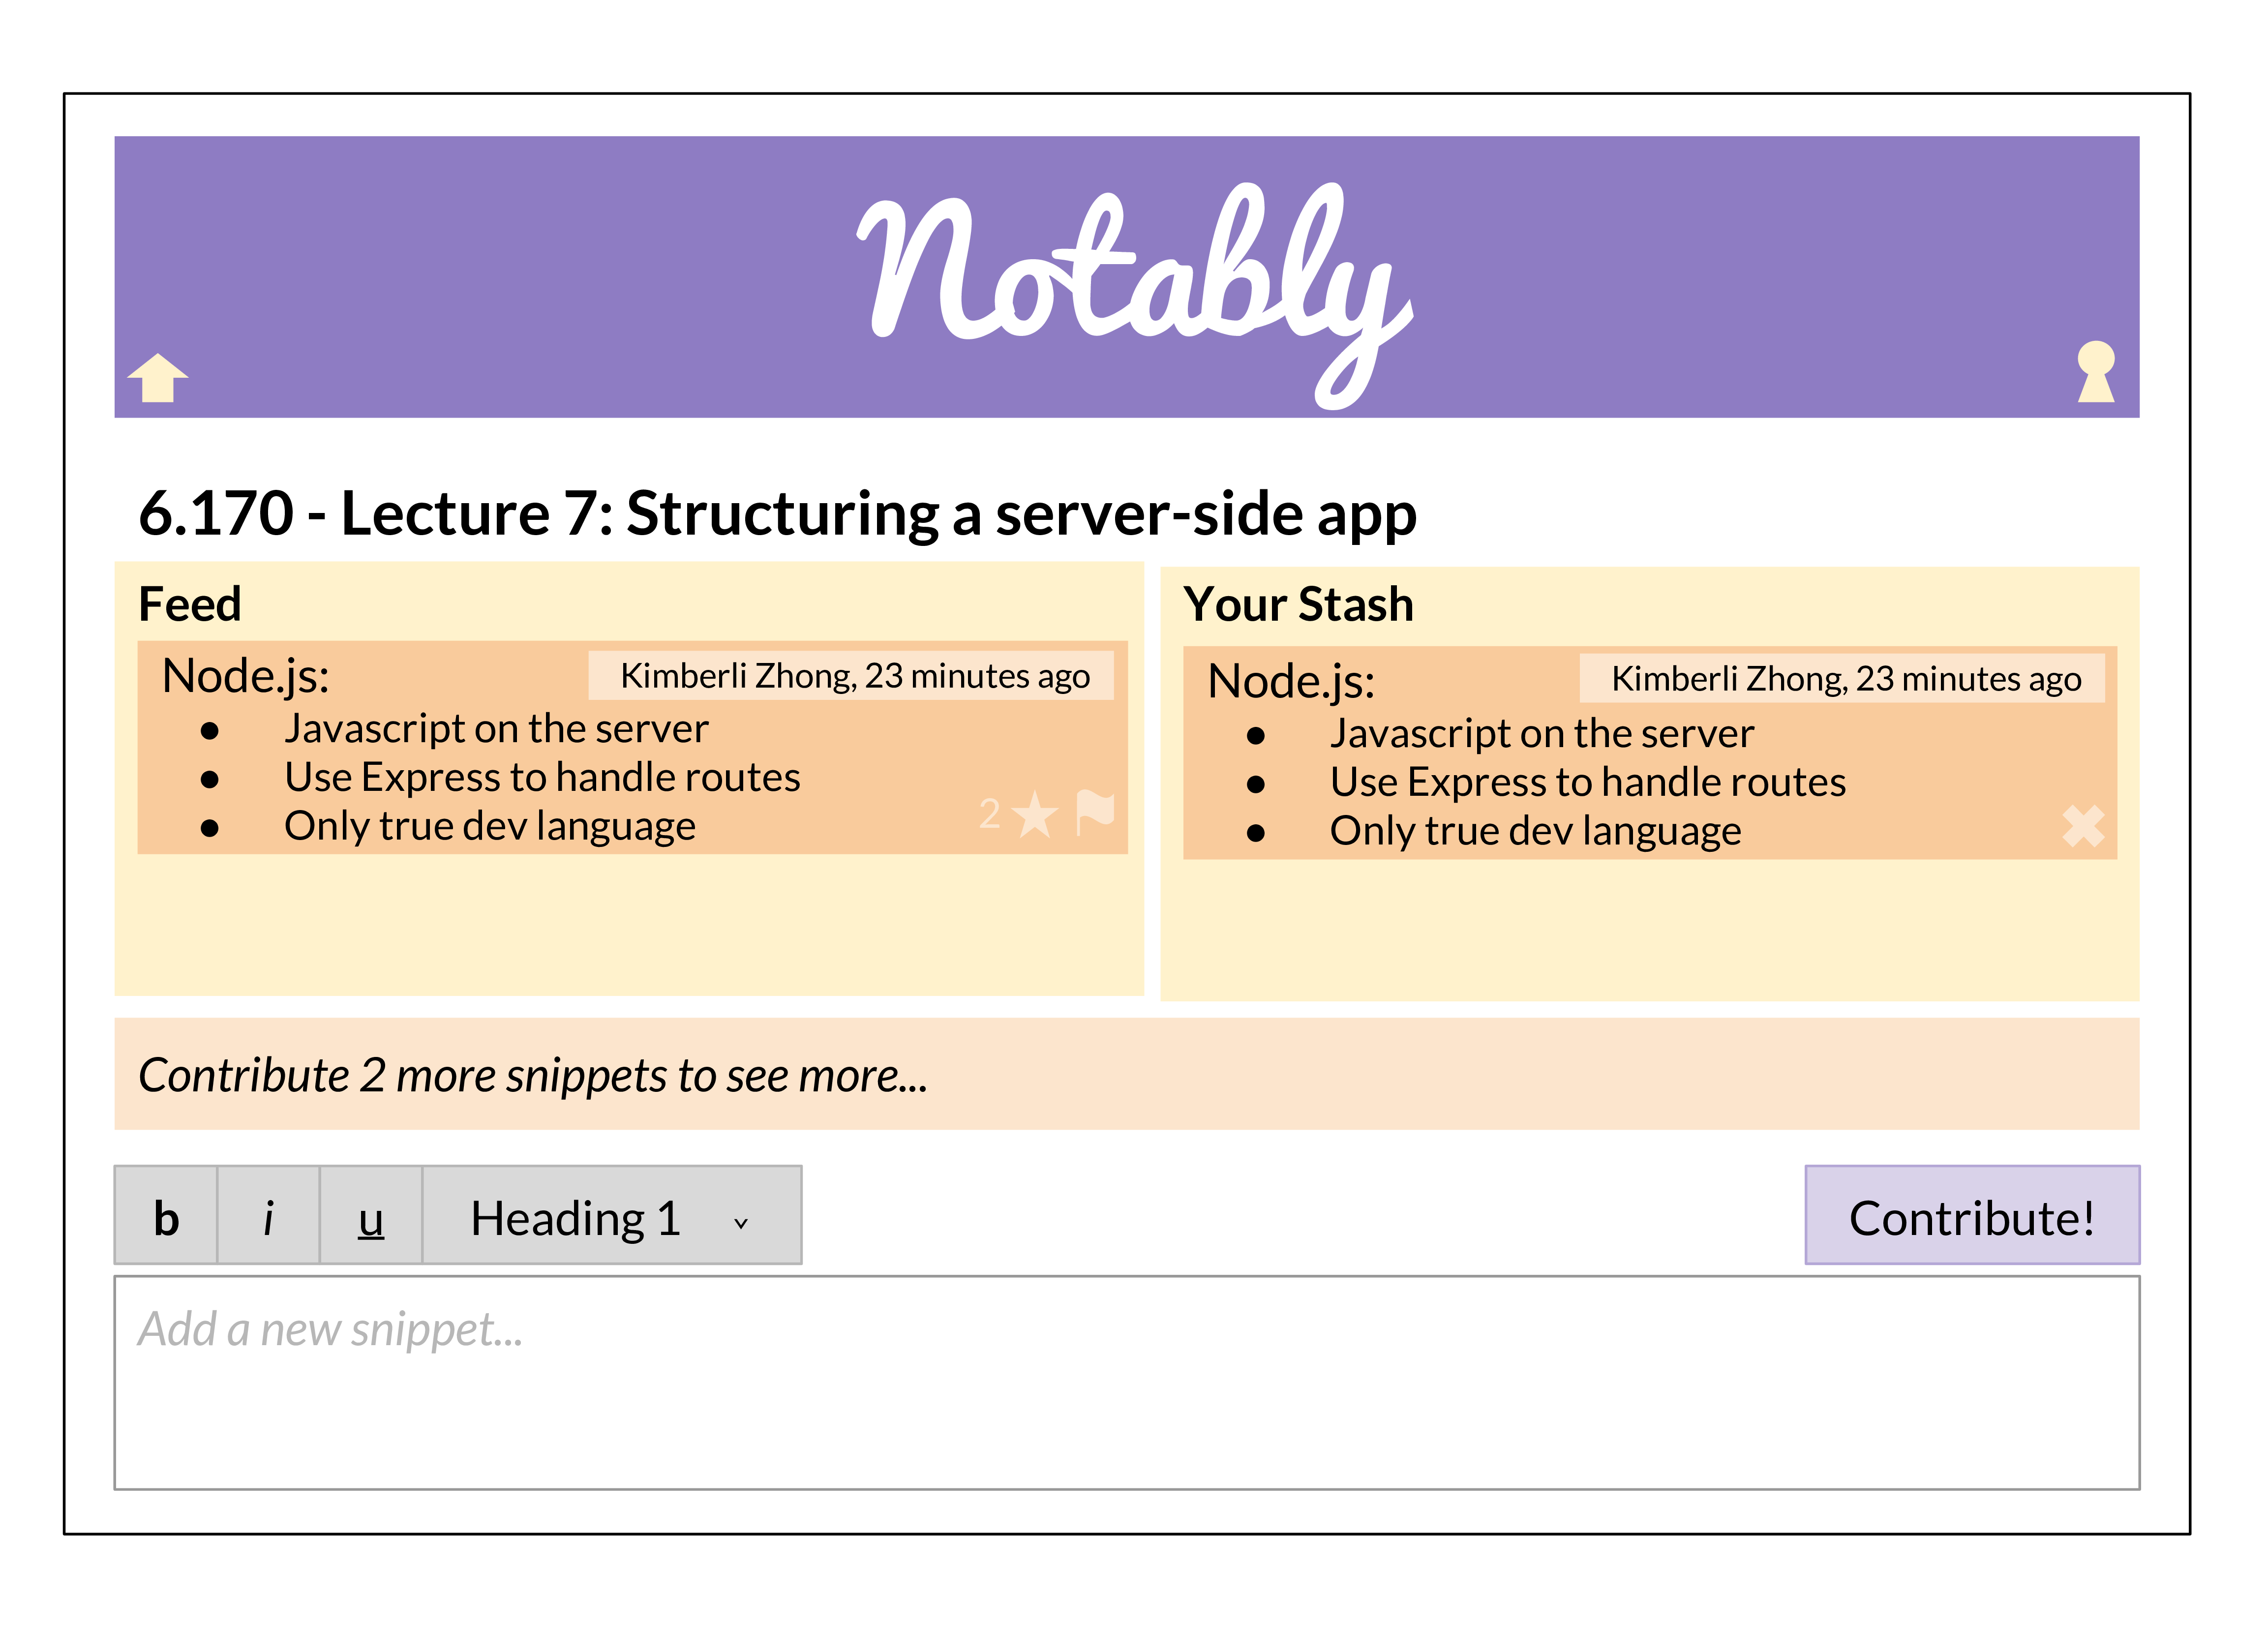
\includegraphics[width=6in]{UI1.png}
\end{figure}

\begin{figure}[h!]
  \caption{Profile view}
  \centering
    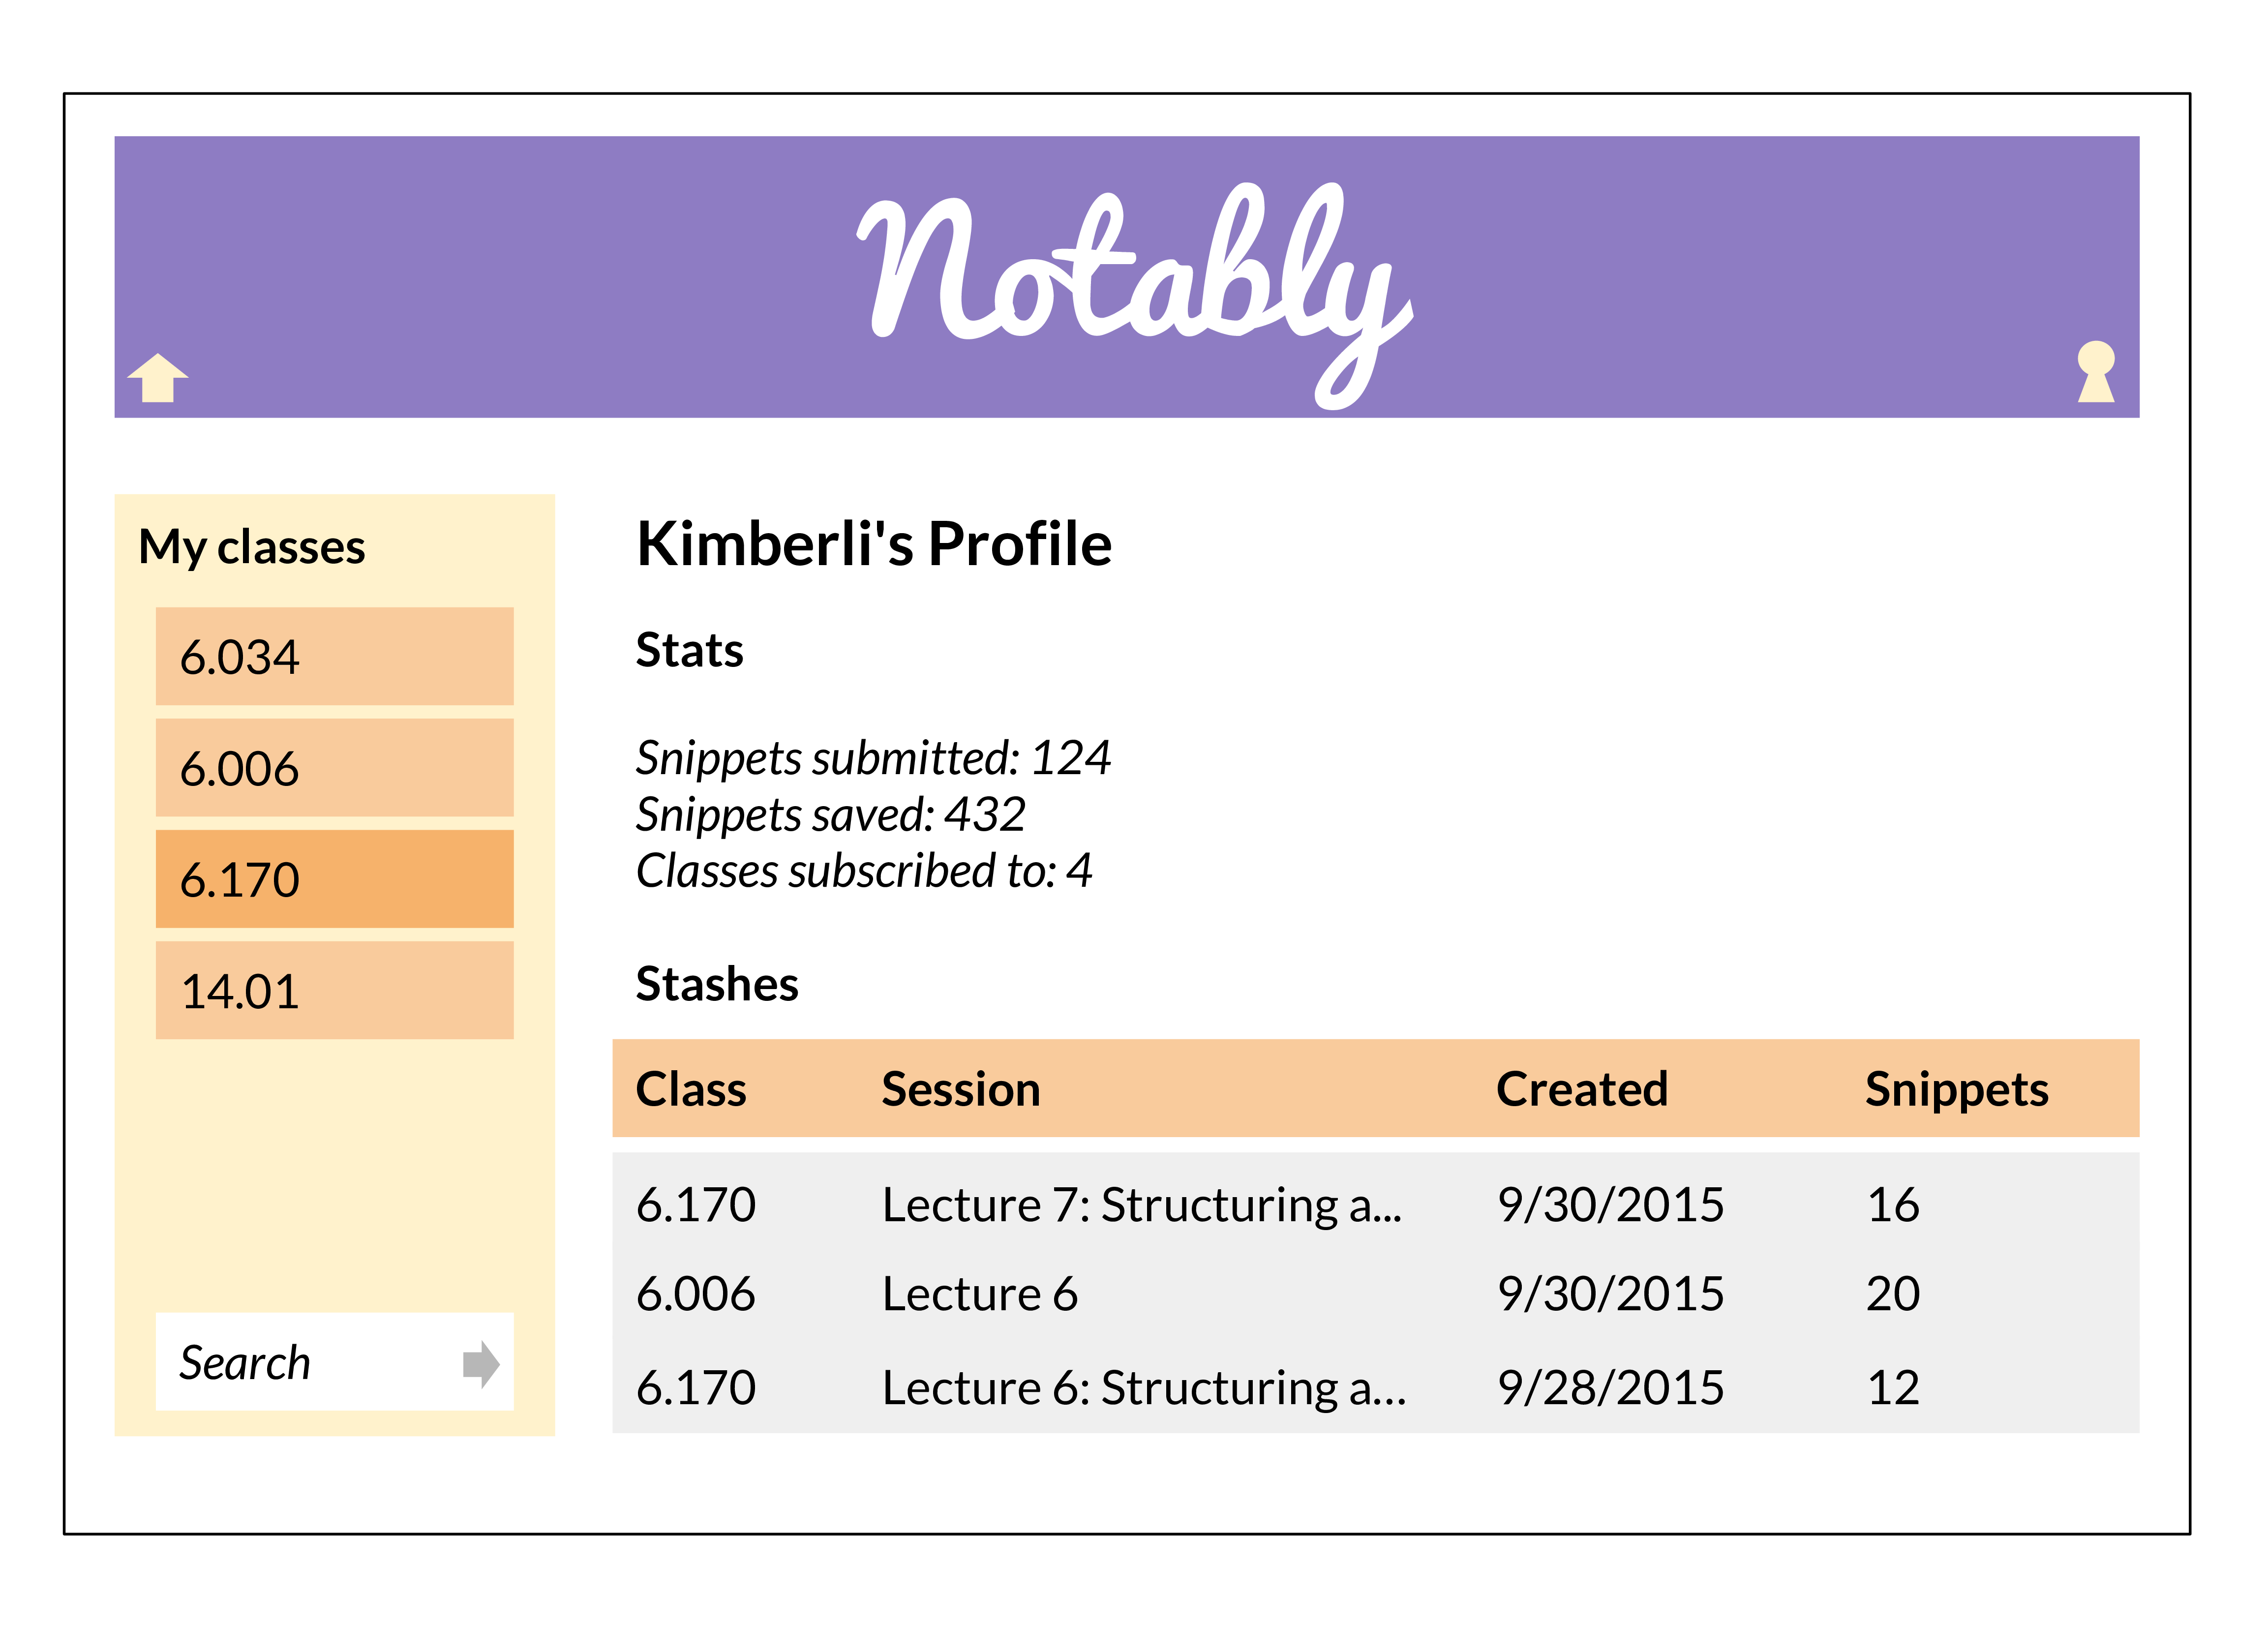
\includegraphics[width=6in]{UI5.png}
\end{figure}

\newpage
% TODO change this:
Upon login with certificate authentication, the user will see a sidebar with options to select her class, and a secondary sidebar (not shown) that will display the sessions for the class. When a session is viewed, the feed for that session is displayed, with snippets obscured when the user hasn't contributed enough. 

The snippet editor features rich text editing and inline math. The system will also have a photo upload option for drawings and graphs. Meanwhile, the feed display shows all snippets for a given session and gives user the option to save snippets to their own stashes or flag snippets as inaccurate.

\section*{Challenges}
\subsection*{Design challenges}
One challenge is deciding whether snippets should be editable. On one hand, it would be nice to be able to fix typos or improve snippets after submitting. On the other hand, we would like to prevent a situation where a user originally stashes a snippet they like, the snippet gets edited, and the user now doesn't want the snippet in their stash. We chose to keep snippets immutable for sake of technical simplicity.

Another challenge is deciding how to administer which feeds exist. Ideally we want everyone in a lecture on the same feed, but also not require users to manually create new feeds (which could result in two users creating feeds for the same lecture). Options include manually creating each feed, creating feeds based on class schedules, and allowing users to manually create feeds. Our solution is to have a pre-existing empty feed that users can contribute to and 3 hours after the first contribution a new feed is automatically created.

Another challenge is deciding the mechanism for unlocking. Our goal is to incentivize contribution by requiring a user to add snippets before having access to the feed, so the feed won't be fully visible right away. At the same time, we want to encourage users to join by immediately showing the benefits of using the system for notes. Our solution is to show the first 10 snippets (as opposed to no snippets) of a feed to anyone and require at least 3 snippets to unlock the rest.

% TEAM WORK PLAN
\section*{Team Work Plan}
\subsection*{Stakeholders}
The stakeholders involved are students as well as instructors and TAs for classes. 

Students can join a particular class, access its feeds, contribute notes, and curate their stashes. The system would provide them an easy way to manage their own study material as well as collaborate and share resources with other students in the class. 

Instructors and TAs are invested in their students' learning and should encourage them to take good notes and learn collaboratively. They can incentivize students to use the app and open up session feeds (lecture, recitation, review session) in which students can contribute notes.

\subsection*{Resources}
MIT Course Catalog: we may need to scrape the course catalog for MIT class metadata. This is a single-time access, and we need not worry about the reliability of the catalog.

\subsection*{Tasks}
The implementation of Notably is divided roughly into the following tasks, along with a tentative point person and deadline:


 \begin{table}[!htbp]
 \centering
\begin{tabular}{|c| l |c|c|}
\hline
\textbf{Category} & \multicolumn{1}{|c|}{\textbf{Task}} & \textbf{Point Person} & \textbf{Deadline} \\
\hline

\multirow{4}{*}{Stack} 
& Certificate Authorization  & Akshay  &  11/19/15 \\\cline{2-4}
& Heroku/Athena    & Vahid  &  11/19/15    \\\cline{2-4}
& MongoDB/Mongolab & Vahid  &  11/19/15    \\\cline{2-4}
& Express/Node  & Vahid  &  11/19/15    \\\cline{2-4}
\hline 

\multirow{5}{*}{Core Functionality} 
& Real-time browser updating  & Akshay  &  11/19/15 \\\cline{2-4}
& Database models    & Alex  &  11/19/15    \\\cline{2-4}
& Client/server communication & Kimberli  &  11/19/15    \\\cline{2-4}
& Save a snippet & Alex  &  11/23/15    \\\cline{2-4}
& Flag a snippet & Akshay  &  12/06/15    \\\cline{2-4}
\hline 

\multirow{4}{*}{Views} 
& Feed View  & Kimberli  &  11/23/15 \\\cline{2-4}
& Stash View  & Alex  &  11/23/15    \\\cline{2-4}
& User Home View (list of stashes)  & Alex  &  11/23/15    \\\cline{2-4}
& Class Home View (list of feeds) & Kimberli  &  11/23/15    \\\cline{2-4}
\hline 

\multirow{4}{*}{Features} 
& List of MIT classes/descriptions  & Akshay  &  12/06/15 \\\cline{2-4}
& Rich Markdown (Text/code formatting, MathJax, etc.)  & Akshay  &  12/06/15    \\\cline{2-4}
& Keyboard shortcuts (list of stashes)  & Kimberli  &  12/06/15    \\\cline{2-4}
& Unlocking  & Akshay  &  12/06/15    \\\cline{2-4}
\hline


\multirow{2}{*}{Testing} 
& Model  & Kimberli  &  12/06/15 \\\cline{2-4}
& UI  & Akshay  &  12/06/15    \\\cline{2-4}
\hline

\multirow{4}{*}{Logistics} 
& Revised Design Document & Whole Team  &  11/19/15 \\\cline{2-4}
& Meeting Agenda & Kimberli  &  per meeting \\\cline{2-4}
& Meeting Progress Report & Alex  &  per meeting \\\cline{2-4}
& Meeting Notes & Alex  &  per meeting \\\cline{2-4}
\hline

\end{tabular}
\end{table}

\newpage

\subsection*{Risks}

A risk is that our moderation system doesn't work as intended and the quality of snippets is low. The result would be that there wouldn't be a strong lure for students to use the app. We can mitigate this by testing and observing instances and properties of desirable and undesirable behavior. We would then implement criteria that allows the desirable behavior while blocking undesirable behavior.

Another risk is that lazy students will abuse the system by using other students' notes to justify not attending class. To prevent this, we mandate that students contribute a few snippets in order to view other students' notes in the session feed.

To allow for students to filter through many potentially redundant notes, we also will implement a rating system in which snippets that are the most popular (saved to most users' stashes) will bubble up to the top of the feed. 

Although the app may need a critical mass for the sharing features to be useful, we intend for the system also offer an elegant way to manage students' personal notes. That way, individuals would be incentivized to use the app even when there aren't too many other users on it. 

\subsection*{Minimum Viable Product}
In our MVP, we expect to have the following features implemented:
\begin{itemize}
\item User and Class home
\item Lecture feed with rudimentary note-taking capabilities
\item Stash and Save Capabilities
\end{itemize}

The MVP includes almost all of the concepts (snippet, stash, feed, save); the missing concepts are flags and unlocking. We will delay certain features of the full product until after the MVP. These include rich text markup in snippets, creating a comprehensive list of MIT classes, and views for user and class home.
\end{document}